\chapter{Einleitung}
\section{Architekturen von neuronalen Netzen}
Der Lernalgorithmus, mit welchem man ein Netz versucht zu trainieren, h�ngt davon ab, wie die Neuronen eines neuronalen Netzes strukturiert sind. Man kann Netz-Architekturen in drei fundamentale Klassen unterscheiden:
\begin{enumerate}
	\item Einschichtige Feedforward Netze
	\item Mehrschichtige Feedforward Netze
	\item Rekurrente Netze
\end{enumerate}

\subsection{Einschichtige Feedforward Netze}
In geschichteten neuronalen Netzen werden die Neuronen in Form von Schichten organisiert. In der einfachsten Form von geschichteten Netzen gibt es eine Input- und eine Outputschicht, wobei die Inputschicht Signale zur Outputschicht, welche die Berechnungen durchf�hrt, sendet und keine umgekehrte Verbindungen existieren. Solche Netze hei�en feedforward- oder azyklische Netze. In Abbildung \ref{single} sehen wir ein Netz mit drei Knoten in der Input- und drei Knoten in der Outputschicht. Ein solches Netz nennt man einschichtig.
\begin{figure}[H]
	\centering
	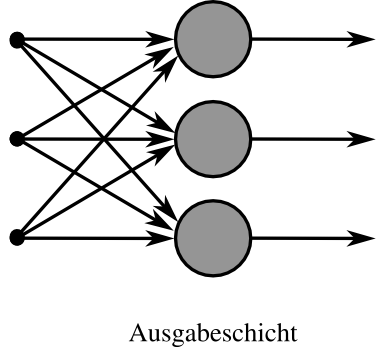
\includegraphics[height=6cm]{SingleLayer.png}
	\caption{SingleLayer Network \itshape(de.wikipedia.org)\upshape}
	\label{single}
\end{figure}

\subsection{Mehrschichtige Feedforward Netze}
Die zweite Klasse der feedforward Netze unterscheidet sich durch eine oder mehrere verdeckte Schichten, deren Knoten zur Berechnung zust�ndig sind und verdeckte Neuronen genannt werden. Ihre Aufgabe ist es, zwischen der Input- und der Outputschicht n�tzlich zu intervenieren. Abbildung \ref{multi} zeigt eine Abbildung eines mehrschichtigen feedforward Netzes mit einer einzelnen verdeckten Schicht mit 3 verdeckten Neuronen.
\begin{figure}[H]
	\centering
	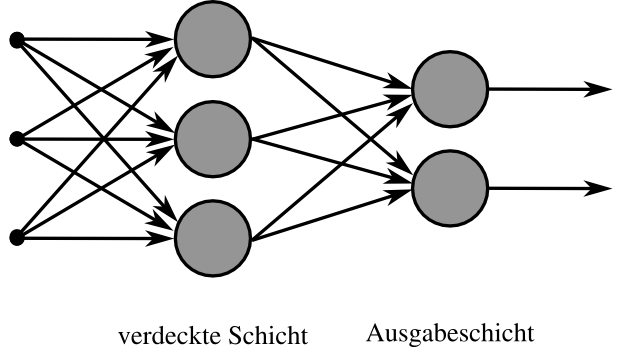
\includegraphics[height=6cm]{MultiLayer.png}
	\caption{MultiLayer Network \itshape(de.wikipedia.org)\upshape}
	\label{multi}
\end{figure}

\subsection{Rekurrente Netze}
Rekurrente Netze sind Neuronale Netze welche sich von den feedforward Netzen unterscheiden, indem sie mindestens eine umgekehrte Verbindung (R�ckkopplung) enthalten, eine sogenannte "`feedback loop"'. Zum Beispiel kann ein rekurrentes Netz (Abbildung \ref{recurrent1}) aus einer Schicht von Neuronen bestehen, welche ihr Outputsignal wieder als Inputsignal verwenden.
\begin{figure}[H]
	\centering
	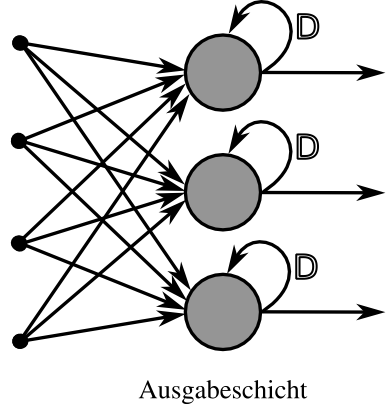
\includegraphics[height=6cm]{Recurrent.png}
	\caption{Recurrent Network 1 \itshape(de.wikipedia.org)\upshape}
	\label{recurrent1}
\end{figure}

Ein anderes Beispiel (Abbildung \ref{recurrent2}) zeigt ein rekurrentes Netz, welches das berechnete Signal der Outputschicht �ber ein zus�tzliches Neuron in der Inputschicht wieder in das Netz einspeist.
\begin{figure}[H]
	\centering
	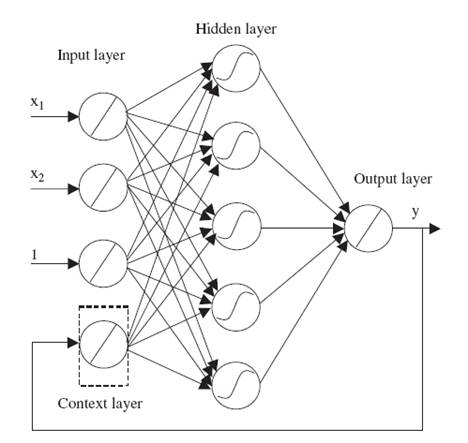
\includegraphics[height=8cm]{Recurrent2.jpg}
	\caption{Recurrent Network 2 \itshape(web.mst.edu)\upshape}
	\label{recurrent2}
\end{figure}

Die Verwendung von "`feedback loops"' hat eine nachhaltige Auswirkung auf die Lernkapazit�t und die Performanz eines Netzes. Meist werden solche umgekehrten Verbindungen zeitlich verz�gert, sodass ein Ged�chtnis und ein dynamisches Verhalten f�r das Netz entsteht.

